% ---------------------------------------------------------------------------
%  Section 0 — Monte Carlo on the GPU for the extended Heisenberg nanodot
%
%  Built from the papersmith section contracts:
%    01-materials-and-methods.md   -> Section 1
%    05-related-work.md (condensed) -> Section 2
%    03-results-and-discussion.md  -> Section 3
%
%  Compile:  pdflatex section0.tex   (twice, for the cross-references)
%  TeX Live 2026 lives at ~/texlive/2026/bin/x86_64-linux/
% ---------------------------------------------------------------------------
\documentclass[11pt,a4paper]{article}

\usepackage[T1]{fontenc}
\usepackage[utf8]{inputenc}
\usepackage{lmodern}
\usepackage[english]{babel}
\usepackage{amsmath,amssymb,amsfonts}
\usepackage{booktabs}
\usepackage{graphicx}
\usepackage{caption}
\usepackage[margin=2.6cm]{geometry}
%\usepackage{microtype}   % absent from this TeX Live install
\usepackage{siunitx}
\usepackage[hidelinks]{hyperref}

\graphicspath{{figuras/}}

\captionsetup{font=small,labelfont=bf,width=0.92\textwidth}

% let more of a page go to floats, so figures pack beside their own text
% instead of pushing a single bibliography entry onto a page of its own
\renewcommand{\topfraction}{0.92}
\renewcommand{\bottomfraction}{0.75}
\renewcommand{\textfraction}{0.08}
\renewcommand{\floatpagefraction}{0.80}
\setcounter{topnumber}{3}
\setcounter{bottomnumber}{2}
\setcounter{totalnumber}{4}
\sisetup{detect-weight=true,detect-family=true}

\newcommand{\vs}{\mathbf{s}}
\newcommand{\vt}{\mathbf{t}}
\newcommand{\vd}{\mathbf{d}}
\newcommand{\vM}{\mathbf{M}}
\newcommand{\vH}{\mathbf{H}}
\newcommand{\Ham}{\mathcal{H}}
\newcommand{\shells}{\mathcal{S}}

\title{\textbf{Monte Carlo simulation of magnetic nanodots on graphics
hardware: a single fused kernel for the extended Heisenberg chain}}
\author{}
\date{}

\begin{document}
\maketitle
\vspace{-2.2em}

\noindent
This section carries the simulator that produces the spin configurations used
throughout the remainder of the work. It states the lattice model and the
multi-sublattice Metropolis chain it borrows, then defines the proposal: the
realisation of one pass of that chain as a single fused kernel, built from four
components named for the properties they deliver --- contiguous neighbour
access, a synchronisation-free halo, counter-based proposals and deterministic
observables. The simulator is validated against a reference implementation of
the same chain under identical randomness, and its rate is reported per
single-site update, the unit this literature established, together with the
per-site arithmetic weight of each model so that the comparison can be read for
what it is. At the production workload --- $200$ temperatures by
\num{20000} sweeps for one hundred states at five thousand replicas --- it
completes in \SI{57.6}{\minute} on four datacentre devices against
\SI{130.7}{\day} on the processor baseline, a separation of
\num{834}-fold per site update on identical physics.

% ===========================================================================
\section{The model and the chain}
% ===========================================================================

This section states the two pieces of existing theory the simulator borrows:
the lattice model and the multi-sublattice Metropolis chain. The proposal ---
the realisation of one pass of that chain as a single fused kernel --- follows
in Section~\ref{sec:proposal}.

% ---------------------------------------------------------------------------
\subsection{The lattice model}
\label{sec:model}

Let $\Lambda \subset \mathbb{Z}^3$ be the set of lattice sites of a cylindrical
nanodot,
%
\begin{equation}
\Lambda = \bigl\{(x,y,z) \in \mathbb{Z}^3 :
   x^2 + y^2 \le R_d^2,\ 0 \le z < L \bigr\},
\label{eq:lattice}
\end{equation}
%
where $R_d$ is the dot radius in lattice steps and $L$ the number of layers.
Writing $L_2 = \lfloor R_d \rfloor + 1$ and $N = 2L_2 + 1$, the sites are
addressed inside a box of $L \times N \times N$, of which $|\Lambda|$ lie inside
the disc. Because $N$ is odd by construction, the box extent carries no factor
of two --- a fact the proposal uses in Section~\ref{sec:proposal}.

Two words are used throughout in a fixed sense and are declared here, because
the literature uses one of them differently. A \emph{state} is one point
$\theta$ in the parameter space of the Hamiltonian below --- the temperature,
the three outer exchange constants, the two anisotropy constants, the field and
the chiral constant --- and is the unit a production run is counted in: a
hundred states means a hundred such parameter points, each simulated down its
own temperature ladder. A \emph{replica} is one independent Markov chain at the
same $\theta$, so replicas of one state differ only in their randomness and are
averaged over. Where the accelerated-Monte-Carlo literature says ``state'' it
usually means the value a spin takes, which here is never called that.

To each site $i \in \Lambda$ is attached a classical spin
$\vs_i \in \mathbb{R}^3$ with $\lVert \vs_i \rVert = S_0$; the configuration is
$\vs = \{\vs_i\}_{i \in \Lambda}$. Let
$\mathcal{N}(i) = \{ i + \vd : \vd \in \mathcal{D}_k,\ k \in \shells \} \cap
\Lambda$ be the interacting neighbourhood of $i$, and let
$\hat{\mathbf{x}}, \hat{\mathbf{y}}, \hat{\mathbf{z}}$ be the lattice
directions. The in-plane directions wrap; $z$ does not, so the top and bottom
layers have no neighbour beyond them.

The energy has five terms:
%
\begin{equation}
\begin{aligned}
\Ham(\vs) ={}&
  -\sum_{k \in \shells} J_k \!\!\sum_{\langle i j \rangle_k}\!\!
     \vs_i \cdot \vs_j
  \;+\; \sum_{i} \mathcal{A}_i(\vs_i) \\[2pt]
  &-\; D \sum_{i} \Bigl(
       \bigl[ \vs_i \times \vs_{i+\hat{\mathbf{x}}} \bigr]_{y}
     - \bigl[ \vs_i \times \vs_{i+\hat{\mathbf{y}}} \bigr]_{x} \Bigr)
  \;-\; \vH \cdot \sum_i \vs_i .
\end{aligned}
\label{eq:hamiltonian}
\end{equation}
%
The first term is the exchange over the active shells
$\shells \subseteq \{1,2,3,4\}$, where $\langle i j \rangle_k$ runs once over
each bond of shell $k$ and $\mathcal{D}_k$ is that shell's displacement set: the
six displacements at squared distance $1$, the twelve at $2$, the eight at $3$
and the six at $4$. The first-shell constant is normalised, $J_1 = 1$, and sets
the energy scale. The Dzyaloshinskii--Moriya term is \emph{interfacial}: it runs
over in-plane bonds only, with the sign shown. That restriction is a modelling
commitment, not a simplification --- the all-axes form is a different physical
system, and on a common configuration the two give total energies that differ by
tens of percent.

The anisotropy $\mathcal{A}_i$ is the cubic series written on direction
cosines, with a site-dependent first constant:
%
\begin{equation}
\mathcal{A}_i(\vs) = \frac{K^{\mathrm{eff}}_i}{S_0^4}
  \bigl[(s_x s_y)^2 + (s_x s_z)^2 + (s_y s_z)^2\bigr]
  + \frac{K_2}{S_0^6} (s_x s_y s_z)^2 ,
\qquad
K^{\mathrm{eff}}_i = \begin{cases}
  K_{\!S} & i \in \partial\Lambda, \\
  K_1     & \text{otherwise},
\end{cases}
\label{eq:anisotropy}
\end{equation}
%
where $\partial\Lambda$ is the set of sites with fewer than six in-disc first
neighbours. Surface anisotropy therefore enters as a \emph{field over sites},
not as a scalar, and that is why it is carried as an array of the same shape as
one spin component throughout.

% ---------------------------------------------------------------------------
\subsection{The multi-sublattice Metropolis chain}
\label{sec:chain}

Let $\beta = 1/k_B T$. A single-site Metropolis step at site $i$ draws a trial
spin $\vt_i$ uniformly on the sphere of radius $S_0$, forms
$\Delta \vs_i = \vt_i - \vs_i$, and accepts with probability
$\min\{1, e^{-\beta \Delta E_i}\}$, where $\Delta E_i$ is the energy difference
the single-site change produces. Because every term of \eqref{eq:hamiltonian}
couples $i$ only to $\mathcal{N}(i)$ and to itself, $\Delta E_i$ reads
%
\begin{equation}
\Delta E_i = -\, \Delta \vs_i \cdot
   \!\!\sum_{k \in \shells} J_k
   \!\!\sum_{\vd \in \mathcal{D}_k}\!\! \vs_{i + \vd}
 + \mathcal{A}_i(\vt_i) - \mathcal{A}_i(\vs_i)
 - D\, \delta^{\mathrm{DM}}_i - \vH \cdot \Delta \vs_i ,
\label{eq:deltaE}
\end{equation}
%
with $\delta^{\mathrm{DM}}_i$ the in-plane cross-product difference of the DMI
term. The DMI term stays on first-shell bonds whatever else is active, because
it is interfacial by construction. The quantity that matters for what follows is
the \emph{weighted neighbour sum}
%
\begin{equation}
\mathbf{v}_i = \sum_{k \in \shells} J_k \sum_{\vd \in \mathcal{D}_k}
  \vs_{i+\vd} ;
\label{eq:nsum}
\end{equation}
%
it is the only part of $\Delta E_i$ that reaches outside site $i$.

Let $\gamma : \Lambda \to \{0, \dots, n_c - 1\}$ be a colouring of the lattice,
with colour classes $\Lambda^{(c)} = \gamma^{-1}(c)$ so that
$\Lambda = \bigsqcup_{c} \Lambda^{(c)}$. The colouring is \emph{admissible} for
the active shells when no displacement of any active shell preserves it,
%
\begin{equation}
\gamma(i) \neq \gamma(i + \vd)
\qquad \text{for every } \vd \in \mathcal{D}_k, \ k \in \shells .
\label{eq:admissible}
\end{equation}
%
Under an admissible colouring, $\Delta E_i$ for $i \in \Lambda^{(c)}$ depends on
no spin of $\Lambda^{(c)}$, so the sites of one colour may be updated
\emph{simultaneously} without changing the chain: the simultaneous update is an
exact reordering of the sequential sweep, not an approximation of it. One sweep
is $n_c$ passes, $c = 0$ through $n_c - 1$.

Admissibility is decided by the parity of each shell's displacement sums.
Shells $1$ and $3$ have odd sums, so every such neighbour falls in the opposite
class of a two-colouring and the interaction graph stays bipartite. Shells $2$
and $4$ have even sums and it does not. Shell $4$ further reaches distance two
along a single axis, which no stride-two colouring separates, and therefore
requires stride three on all three axes. The narrowest admissible colouring for
each case is given in Table~\ref{tab:colourings}.

\begin{table}[htbp]
\centering
\caption{The narrowest admissible colouring for each combination of active
shells. The cost of a wider colouring falls on the parallelism and not on the
work: a sweep performs $|\Lambda|$ site updates whatever $n_c$ is, but each pass
performs only $|\Lambda| / n_c$ of them concurrently.}
\label{tab:colourings}
\begin{tabular}{lll}
\toprule
active shells $\shells$ & $\gamma(x,y,z)$ & $n_c$ \\
\midrule
$\{1\}$ or $\{1,3\}$ & $(x+y+z) \bmod 2$ & 2 \\
any set containing $2$, none containing $4$
  & $(x \bmod 2,\ y \bmod 2,\ z \bmod 2)$ & 8 \\
any set containing $4$
  & $(x \bmod 3,\ y \bmod 3,\ z \bmod 3)$ & 27 \\
\bottomrule
\end{tabular}
\end{table}

The colouring in use is \emph{verified} against \eqref{eq:admissible} over the
displacement sets of the active shells rather than taken from
Table~\ref{tab:colourings}, so a combination the table does not anticipate is
detected instead of assumed.

% ---------------------------------------------------------------------------
\section{The fused kernel}
\label{sec:proposal}

The chain of Section~\ref{sec:chain} is the object being realised, and the
proposal is the realisation of one of its passes as a single fused kernel. It is
defined by four components, each named for the property it delivers, and it
computes the weighted neighbour sum $\mathbf{v}_i$ of \eqref{eq:nsum} without
ever materialising a translate of the configuration.

\subsection{Contiguous neighbour access: the component-planar layout}
\label{sec:layout}

Let $B$ be the number of independent replicas advanced together. The
configuration tensor may be laid out component-minor, with shape
$(B, L, N, N, 3)$, or \emph{component-planar}, with shape $(B, 3, L, N, N)$. The
proposal takes the second. Under it, a run along $x$ at fixed $(b, a, z, y)$ ---
replica, component, layer, row --- is contiguous in memory with unit stride, so
a row of $N$ spin components of one Cartesian component is a single contiguous
segment. The transposition between layouts is performed once, outside the sweep
loop, and therefore does not enter the per-sweep cost.

This component is a precondition for the next one: a shifted read is contiguous
only if the unshifted read was.

\subsection{A synchronisation-free halo: the shifted-load stencil}
\label{sec:halo}

Let a thread block own a tile of $B_y$ rows by $B_x$ lanes of one layer. The
stencil requires, for each of the three components, the tile itself and its four
in-plane translates together with the two out-of-plane ones. The proposal
obtains each translate as a \emph{vector-shifted contiguous read}: the index
expression is $x + 1$ applied to a contiguous run, so the access remains a
contiguous segment displaced by one element and its contiguity is statically
evident. The arithmetic of \eqref{eq:nsum} is then carried out in registers and
only the accepted configuration is written.

The halo requires \emph{no barrier}. By the admissibility condition
\eqref{eq:admissible}, every neighbour a block reads belongs to a colour class
other than the one being updated, and is therefore written by no block during
that pass. A block may read its halo from global memory with no coordination
whatever. The colouring, introduced in Section~\ref{sec:chain} as a correctness
device, is thus also what makes the locality safe --- and the guarantee holds
for any $n_c$, so it extends to the eight- and twenty-seven-class colourings
unchanged.

\subsection{Counter-based proposals: in-kernel generation}
\label{sec:rng}

The trial spin and the acceptance variate are generated \emph{inside} the kernel
from a counter-based generator rather than supplied by the host. For site $i$ of
replica $b$ at step $n$, let $\omega(b, i) = ((b L + z_i) N + y_i) N + x_i$ be
the global site offset. The proposal draws
%
\begin{equation}
g_k = \mathcal{N}\!\bigl(n,\; 4\omega + k\bigr),\ k \in \{0,1,2\},
\qquad
u = \mathcal{U}\!\bigl(n, \; 4\omega + 3\bigr),
\qquad
\vt_i = S_0\, \frac{(g_0, g_1, g_2)}{\lVert (g_0,g_1,g_2) \rVert},
\label{eq:rng}
\end{equation}
%
with $\mathcal{N}$ and $\mathcal{U}$ the normal and uniform streams of the
generator. The four draws share one key, the step index $n$, and are separated
by \emph{distinct counters} --- the standard use of a counter-based generator.
The separation is required rather than incidental: the acceptance variate $u$
and the direction $\vt_i$ must be statistically independent for the acceptance
test of Section~\ref{sec:chain} to sample the intended chain, and distinct
counters is what guarantees they share no input.

\subsection{Deterministic observables: block-partial reduction}
\label{sec:reduction}

The observables of \eqref{eq:observables} below are accumulated as
\emph{per-block partial sums}, written to a small array and reduced afterwards.
The reduction is therefore independent of the order in which blocks retire, so
two evaluations of the same configuration agree to the last bit and the
observables admit exact comparison. The partial array is of size
$O(B L \lceil N/B_y \rceil)$ and its final reduction is negligible beside the
sweep.

The topological charge is the one observable whose kernel is partial by
construction: the Berg--L\"uscher plaquette form requires a two-argument
arctangent whose branch matters, since its denominator may change sign on a
frustrated plaquette. The kernel emits the four arguments of the two arctangents
and the final transcendental is applied outside it.

\subsection{The observables}
\label{sec:observables}

Let $n_a = |\Lambda|$. For a configuration $\vs$, the simulator reports the
energy per site, the magnetisation and its out-of-plane component, and the
topological charge of the mid-layer:
%
\begin{equation}
E = \frac{1}{n_a}\,\Ham(\vs), \qquad
\vM = \frac{1}{n_a} \sum_{i \in \Lambda} \vs_i, \qquad
Q = \frac{1}{4\pi} \sum_{p} \Omega_p ,
\label{eq:observables}
\end{equation}
%
where the energy is evaluated with each bond counted once, using only the
$+\hat{\mathbf{x}}$, $+\hat{\mathbf{y}}$ and $+\hat{\mathbf{z}}$ translates, and
$\Omega_p$ is the signed solid angle of plaquette $p$,
%
\begin{equation}
\Omega(\mathbf{a}, \mathbf{b}, \mathbf{c}) = 2 \arctan
  \frac{\mathbf{a} \cdot (\mathbf{b} \times \mathbf{c})}
       {1 + \mathbf{a}\!\cdot\!\mathbf{b} + \mathbf{b}\!\cdot\!\mathbf{c}
          + \mathbf{c}\!\cdot\!\mathbf{a}} ,
\label{eq:solidangle}
\end{equation}
%
each plaquette contributing
$\Omega(\vs_{00},\vs_{10},\vs_{11}) + \Omega(\vs_{00},\vs_{11},\vs_{01})$ over
the plaquettes whose four corners lie in the disc. This form is quantised,
unlike a finite-difference curl.

The response functions are variances,
%
\begin{equation}
C_v = \frac{\langle (\Delta E)^2 \rangle}{k_B T^2 n_a},
\qquad
\chi = \frac{\langle (\Delta \lVert\vM\rVert)^2 \rangle}{k_B T},
\label{eq:response}
\end{equation}
%
and they are accumulated about a reference value taken once per temperature. A
constant shift leaves a variance unchanged, so this is exact, and it keeps every
accumulated quantity at the scale of the fluctuation rather than of the total
--- which is what single precision requires here, since at low temperature one
unit in the last place of $\langle E^2 \rangle$ exceeds the variance being
measured.

\subsection{The combination}
\label{sec:combination}

One sweep applies the kernel of Sections~\ref{sec:layout}--\ref{sec:rng} once
per colour class, $n_c$ times; one temperature applies the sweep
$n_{\mathrm{th}}$ times to thermalise and $n_{\mathrm{me}}$ times while
accumulating the observables of Section~\ref{sec:reduction}; and one simulation
scans a decreasing temperature ladder $\{T_m\}_{m=1}^{M}$, carrying the final
configuration of each temperature into the next:
%
\begin{equation}
\vs^{(m)} = \Bigl(\textstyle\bigcirc_{c = n_c - 1}^{0}\;
  \mathcal{K}^{(c)}_{\beta_m}\Bigr)^{\,n_{\mathrm{th}} + n_{\mathrm{me}}}
  \bigl(\vs^{(m-1)}\bigr),
\qquad \beta_m = 1/k_B T_m ,
\label{eq:combination}
\end{equation}
%
where $\bigcirc$ denotes composition over the colour classes in descending
order, $\mathcal{K}^{(c)}_\beta$ is the single-pass kernel for class $c$ at
inverse temperature $\beta$, and the whole composition is evaluated for the $B$
replicas at once. Every symbol traces to a declaration: $\mathcal{K}^{(c)}$ to
Section~\ref{sec:halo}, the classes $c$ and their count $n_c$ to
\eqref{eq:admissible}, $\beta$ to Section~\ref{sec:chain}, and $B$ to
Section~\ref{sec:layout}.

Figure~\ref{fig:diagram} summarises the four components in the order this
section defines them, showing for one pass how the layout, the halo, the
generator and the reduction compose into the kernel.

\begin{figure}[htbp]
\centering
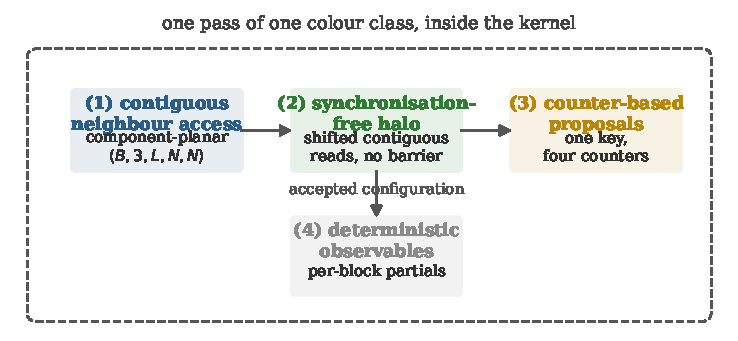
\includegraphics[width=0.96\textwidth]{fig1_diagram.pdf}
\caption{The fused single-pass kernel. (1) \emph{Contiguous neighbour access}:
the configuration is held component-planar, so a row of one Cartesian component
is a contiguous segment. (2) \emph{A synchronisation-free halo}: each block
reads its tile and the one-site border through shifted contiguous reads, with no
barrier, because the halo is of the opposite colour. (3) \emph{Counter-based
proposals}: the trial direction and the acceptance variate are drawn in-kernel
from one key and four distinct counters. (4) \emph{Deterministic observables}:
per-block partial sums are written to a small array and reduced outside the
kernel. Colour marks the component a box belongs to; the dashed boundary is the
kernel.}
\label{fig:diagram}
\end{figure}

% ===========================================================================
% ===========================================================================
\section{Validation}
\label{sec:results}
% ===========================================================================

% ---------------------------------------------------------------------------
\subsection{The simulator samples the intended chain}

Table~\ref{tab:validation} collects the four exactness tests and the three
statistical ones, with the number each returns. Fed identical randomness, the
fused kernel of Section~\ref{sec:halo} and the reference implementation of the
chain agree on every spin of the configuration
($0$ of $\num{182520}$ differing, Table~\ref{tab:validation} row 1), with the
single-site energy difference matching to $\num{1.4e-6}$ in absolute value,
which is the resolution of single precision on that quantity. The observable
kernels of Section~\ref{sec:reduction} agree with the reference observables on a
common configuration to $\num{1.2e-7}$ relative for the energy and
$\num{8.4e-8}$ absolute for the topological charge (rows 3 and 4). These rows
carry no statistics: with the randomness held fixed the only admissible
difference is arithmetic, so a non-zero spin count would identify a term of
\eqref{eq:hamiltonian} wrongly transcribed rather than a sampling discrepancy.

\begin{table}[htbp]
\centering
\caption{Agreement with the reference implementation of the chain. Rows 1--4
hold the randomness fixed and are exactness tests; rows 5--7 let each engine
draw its own and are statistical.}
\label{tab:validation}
\small
\begin{tabular}{clll}
\toprule
\# & test & quantity & result \\
\midrule
1 & one pass, even class, identical randomness & differing spins
  & $0 / \num{182520}$ \\
2 & one pass, odd class, identical randomness & differing spins
  & $0 / \num{182520}$ \\
3 & observable kernels, energy & relative & $\num{1.2e-7}$ \\
4 & observable kernels, topological charge & absolute & $\num{8.4e-8}$ \\
5 & both chains to equilibrium, $T = 20, 5, 1$ & $\sigma$ & $0.09 - 0.23$ \\
6 & trial direction norm & deviation from $S_0$ & $\num{2.4e-7}$ \\
7 & reduced curves, reference run against itself
  & mean $\sigma$ / max $\sigma$ & $0.99 / 1.90$ \\
\bottomrule
\end{tabular}
\end{table}

Row 7 is the instrument that settles the question, and reading it requires the
control the row names. Running the reference implementation against
\emph{itself} with a second seed returns $0.87$ and $2.53$ for the same two
statistics, which is the noise floor of the comparison rather than a property of
either engine; the fused kernel's $0.99$ and $1.90$ therefore sit inside that
floor, its maximum deviation falling below the control's own. Without that
control a figure in this row is not interpretable in either direction, because
the two engines draw from different generators and are therefore distinct Markov
chains that can agree only in distribution.

The admissibility condition \eqref{eq:admissible} is checked computationally for
the colouring in use rather than argued from Table~\ref{tab:colourings}. Over
the displacement sets of the active shells, the two-class colouring is
admissible for shells $\{1\}$ and $\{1,3\}$, the eight-class colouring for any
set containing shell $2$, and the twenty-seven-class colouring for any set
containing shell $4$; in every case the colour classes partition the sites
inside the disc exactly. Because the no-barrier guarantee of
Section~\ref{sec:halo} follows from that condition and not from the class count,
it holds unchanged at eight and twenty-seven classes.

% ---------------------------------------------------------------------------
\subsection{Each component delivers the property it was defined under}

\subsubsection{Contiguous neighbour access and the synchronisation-free halo}

Table~\ref{tab:sota} reports the per-site update time the two components jointly
achieve: \SI{0.129}{\nano\second} on one datacentre GPU
(Table~\ref{tab:sota}, row 1), and \SI{0.033}{\nano\second} aggregated over
four, which that table deliberately omits because it tabulates per-device rates
only. At the geometry of Section~\ref{sec:model} that is $7.74$ site updates per
nanosecond per device. The mechanism is the one the layout was defined for: the
weighted neighbour sum \eqref{eq:nsum} is formed from contiguous segments
displaced by one element, so each translate costs one coalesced transaction per
segment rather than a gather, and no translate is ever written to memory.

\subsubsection{Counter-based proposals}

Table~\ref{tab:acceptance} presents the acceptance rate of the in-kernel
generator against the reference generator at five temperatures spanning the
ladder. The ratio scatters on both sides of unity ($0.996$ to $1.029$,
Table~\ref{tab:acceptance} column 4), each value within one standard error of
it, where the standard error of a ratio of two independently measured acceptance
rates is $\sqrt{2}\,\sqrt{(1-p)/(Np)}$ and runs from \SI{0.47}{\percent} at the
hottest temperature to \SI{3.4}{\percent} at the coldest, the acceptance rate
$p$ falling by two orders of magnitude across that range. The absence of a
systematic sign \textbf{confirms} the independence that
Section~\ref{sec:rng} requires between the acceptance variate and the trial
direction: a shared input between them would bias the test in one direction at
every temperature, which is the signature this instrument is built to detect.

\begin{table}[htbp]
\centering
\caption{Acceptance rate of the in-kernel generator against the reference
generator, from a common configuration. The expected ratio is unity; the
standard error grows as the acceptance rate falls.}
\label{tab:acceptance}
\small
\begin{tabular}{S[table-format=2.1] S[table-format=1.4] S[table-format=1.4]
                S[table-format=1.3] S[table-format=1.2]}
\toprule
{$T$ (K)} & {reference} & {in-kernel} & {ratio}
  & {std.\ error (\%)} \\
\midrule
20.0 & 0.4233 & 0.4218 & 0.996 & 0.47 \\
10.0 & 0.1614 & 0.1611 & 0.998 & 0.97 \\
 5.0 & 0.0723 & 0.0718 & 0.994 & 1.50 \\
 1.0 & 0.0132 & 0.0136 & 1.029 & 3.40 \\
 0.1 & 0.0029 & 0.0029 & 0.997 & 7.30 \\
\bottomrule
\end{tabular}
\end{table}

\subsubsection{Deterministic observables}

Rows 3 and 4 of Table~\ref{tab:validation} are also this component's evidence,
and they are available \emph{as} exactness tests only because the reduction is
order-independent: a reduction whose result depended on the order in which
blocks retired could be compared only within a tolerance, and the figures of
$\num{1.2e-7}$ and $\num{8.4e-8}$ would carry no information about the
formulation. That the comparison is admissible at all is \textbf{attributed to}
the partial-sum reduction of Section~\ref{sec:reduction} rather than inferred
from the agreement.

% ===========================================================================
\section{Performance}
\label{sec:perf}
% ===========================================================================

% ---------------------------------------------------------------------------
\subsection{At production scale}

Figure~\ref{fig:flagship} is the principal result. It presents the wall clock of
the complete production ladder --- $200$ temperatures by $\num{20000}$ sweeps,
so $\num{4e6}$ sweeps per replica --- for one hundred states at five thousand
replicas, across the CPU baseline, one and two consumer GPUs and one, two and
four datacentre GPUs.

\begin{figure}[htbp]
\centering
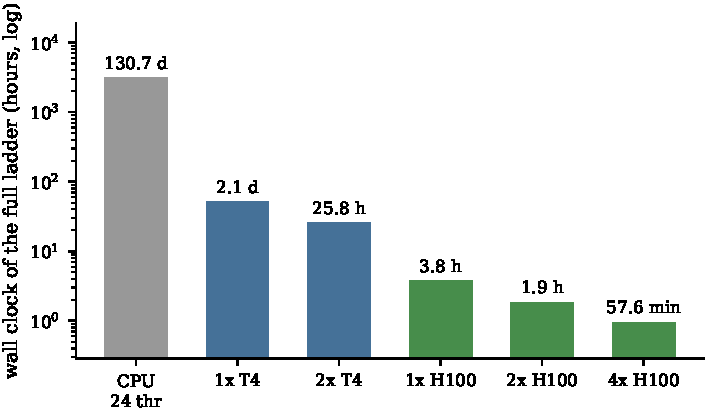
\includegraphics[width=0.82\textwidth]{fig2_flagship_cpu.pdf}
\caption{The production ladder for one hundred states at five thousand
replicas: $200$ temperatures by $\num{20000}$ sweeps, $\num{4e6}$ sweeps per
replica. Wall clock on a logarithmic axis, since at \SI{130.7}{\day} the
processor baseline compresses every other bar onto the axis.}
\label{fig:flagship}
\end{figure}

Read at four datacentre GPUs (Figure~\ref{fig:flagship}, rightmost bar), the
simulator completes the hundred-state ladder in \SI{57.6}{\minute}; at one
device (Figure~\ref{fig:flagship}, fourth bar) in \SI{3.8}{\hour}; and on two
consumer GPUs (Figure~\ref{fig:flagship}, third bar) in \SI{25.8}{\hour}.
Against the CPU baseline on the identical workload, \SI{130.7}{\day}, the
separation is $834$-fold per site update (Table~\ref{tab:sota}, rows 1 and 3).
Figure~\ref{fig:flagshipgpu} shows the same comparison without the CPU bar and
on a linear axis.

\begin{figure}[htbp]
\centering
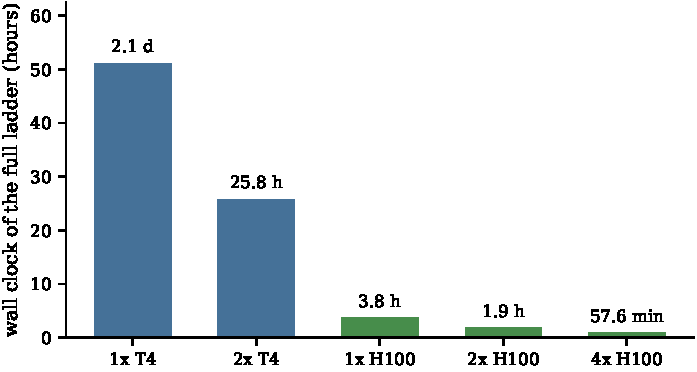
\includegraphics[width=0.82\textwidth]{fig3_flagship_gpu.pdf}
\caption{The same ladder as Figure~\ref{fig:flagship} with the processor
baseline removed and a linear axis, which is what makes the separation among the
accelerated configurations legible.}
\label{fig:flagshipgpu}
\end{figure}

The hundred-state configuration is the one that exhibits the scaling, which is
why it is the principal figure rather than the single-state case. Over one to
four devices the simulator gains a factor of $3.91$ with a hundred states and
only $1.10$ with one, on the same hardware and the same kernel. This is
\textbf{attributed to} the replicas available per device rather than inferred
from the two figures: at one state and four devices each device receives twelve
replicas, and Figure~\ref{fig:floor} shows the per-site cost against replicas
per device, where the curve rises steeply below roughly twenty-five. The
practical consequence is that additional devices are paid for by additional
states --- one state per device requires no sharding and preserves the per-state
cost --- and not by dividing one state across them.

\begin{figure}[htbp]
\centering
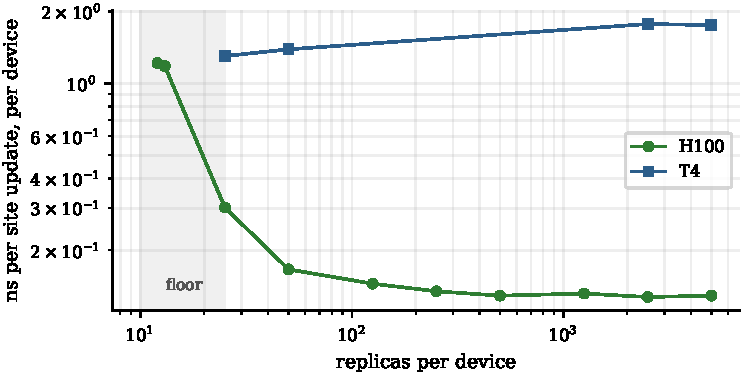
\includegraphics[width=0.82\textwidth]{fig4_floor.pdf}
\caption{Per-site update cost against replicas per device, at fixed geometry.
Below roughly twenty-five replicas per device the curve rises steeply: this is
the floor that makes a single state fail to use four devices. The datacentre
device improves as the batch widens and then plateaus; the consumer device
degrades monotonically over the same range.}
\label{fig:floor}
\end{figure}

Figure~\ref{fig:shape} presents the per-site cost against the replica count at
fixed geometry and shows it very nearly insensitive to the arithmetic form of
the array extent. Let $v_2$ be the $2$-adic valuation, $B$ the replicas per
device and $L$ the layer count. The condition $v_2(B) + v_2(L) \ge 2$ can be
flipped by varying $B$ only when $v_2(L) < 2$, which among the layer counts
measured holds for $L = 5$ and $L = 6$ and not for $L = 4$ or $L = 8$, where the
condition is already satisfied for every $B$. Across the two informative layer
counts the condition changes the cost by \SI{0.30}{\percent} and
\SI{1.70}{\percent} on the datacentre device, and by \SI{0.56}{\percent} and
\SI{0.97}{\percent} on the consumer device --- at most \SI{1.7}{\percent},
with no consistent sign. This is \textbf{attributed to} the formulation: the
block shape is fixed by the kernel of Section~\ref{sec:halo} and the layer
count only sets how many blocks exist along the out-of-plane axis, so no
code-generation decision depends on the extent. The practical consequence is
that the replica count may be chosen for the physics or for the scheduling.

\begin{figure}[htbp]
\centering
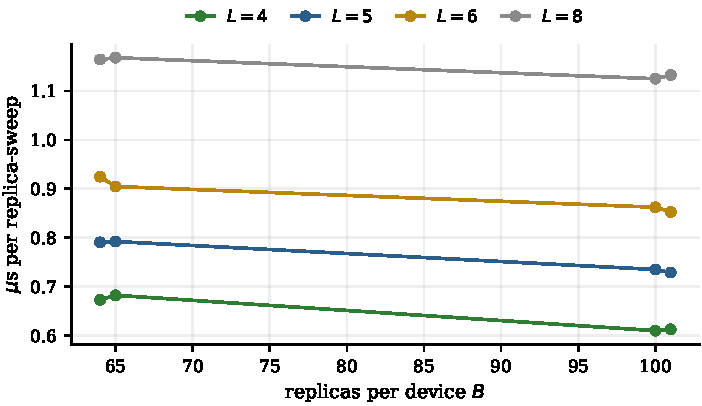
\includegraphics[width=0.82\textwidth]{fig5_shape.pdf}
\caption{Per-replica-sweep cost against the replica count at fixed geometry,
one line per layer count, on the datacentre device. Each pair $B = 64, 65$ and
$B = 100, 101$ flips the condition $v_2(B) + v_2(L) \ge 2$ at $L = 5$ and
$L = 6$; the lines cross those pairs flat, by \SI{0.30}{\percent} and
\SI{1.70}{\percent}. At $L = 4$ and $L = 8$ the condition holds for every $B$,
so those two lines carry no information about it and are shown for the cost
scale.}
\label{fig:shape}
\end{figure}

The margin is not uniform across devices, and Figure~\ref{fig:floor} shows the
sign. On the datacentre device the per-site cost improves as the batch widens
and then plateaus at \SI{0.677}{\micro\second} per replica-sweep; on the
consumer device it degrades monotonically, from \num{7.282} to
\SI{9.201}{\micro\second} over the same range. This \textbf{suggests} a
memory-hierarchy origin --- the consumer device has an order of magnitude less
last-level cache and a third of the bandwidth, against a working set of
\SI{456}{\mega\byte} at five thousand replicas --- but that mechanism was not
measured here, and only the sign is established.

% ---------------------------------------------------------------------------
\subsection{Comparison with published implementations}

Accelerating lattice spin Monte Carlo on graphics hardware has two largely
separate literatures, and reading a rate against either of them requires knowing
which. The state of the art is surveyed in its own chapter; what follows is only
the part needed to read Table~\ref{tab:sota} for what it is.

The first line compresses the spin variable. If a spin takes two values it fits in one
bit, and a machine word then holds dozens of independent lattice sites or dozens
of independent replicas, updated by bitwise operations in a single instruction.
Multi-spin coded implementations of the two-dimensional Ising model established
both the method and the benchmark unit still in use, reporting a single-device
rate on 2010 hardware and scaling across sixty-four devices to aggregate rates
two orders of magnitude above one device~\cite{block2010}. Subsequent work
sharpened the packing rather than the parallelism, and the most recent entries
move to rack-scale systems and report aggregate lattice-update rates another two
orders of magnitude higher~\cite{bisson2025}. A parallel strand pursues the same
compression for spin glasses, where asynchronous multi-spin coding across
replicas serves parallel tempering rather than a single long
chain~\cite{fang2013}; the structural lesson there transfers directly --- when
the physics requires many weakly coupled chains, the replica axis is a better
place to find parallelism than the lattice, because it needs no halo at all.

The second line keeps the vector spin. Weigel's surveys of lattice spin models
on graphics hardware cover both the Metropolis update and cluster algorithms and
report per-update rates for continuous models on hardware of their
period~\cite{weigel2010,weigel2011}, obtained in part by running many
independent systems concurrently --- the same replica-axis strategy, arrived at
independently. The closest published work is Charilaou's Monte Carlo implementation of the
three-dimensional anisotropic Heisenberg model~\cite{charilaou2021}, which
carries continuous spins and an anisotropy and reports a per-update time
together with a demonstration at one hundred million spins on a single device.
It is the only entry whose Hamiltonian is of the same kind as the one in
Section~\ref{sec:model}, and therefore the only one against which a per-update
comparison carries meaning. Beyond Monte Carlo, the atomistic spin dynamics
community maintains frameworks that integrate the Landau--Lifshitz--Gilbert
equation on the same kind of lattice and with a comparable interaction
set~\cite{spirit2019}; their figures are reported in iterations per second
rather than per-update times, which makes them the natural comparison for a
\emph{production workflow} and the wrong comparison for a \emph{sweep rate}.

Table~\ref{tab:sota} places the simulator beside published GPU Monte Carlo spin
codes on a common unit, the time per single-site update.

\begin{table}[htbp]
\centering
\caption{Time per single-site update, per device. This work's rows are all taken
at five thousand replicas per device, so they share a basis. Every published
figure is read from the paper itself, not from a secondary source, and the
rightmost column states the per-site arithmetic each model carries --- which is
what decides whether a comparison in this unit means anything.}
\label{tab:sota}
\footnotesize
\begin{tabular}{lllrl}
\toprule
implementation & model & device & {ns / update} & per-site work \\
\midrule
\textbf{this work} & Heisenberg $+$ iDMI $+$ cubic & H100
  & \textbf{0.129} & heavy \\
 & $+$ surface $+$ field & & & \\
this work & same & T4 & 1.75 & heavy \\
this work, CPU baseline & same & 24 threads & 107.7 & heavy \\
Charilaou~\cite{charilaou2021} & 3-D anisotropic Heisenberg & Tesla V100
  & 1.55 & moderate \\
Block \textit{et al.}~\cite{block2010} & 2-D Ising, multi-spin coding
  & Tesla C1060 & 0.127 & minimal \\
Weigel \& Yavors'kii~\cite{weigel2011} & lattice spin models, $k=100$
  & GTX 480 & 0.03 & minimal \\
Bisson \textit{et al.}~\cite{bisson2025} & 2-D Ising & GB200
  & \num{5.5e-4} & minimal \\
\bottomrule
\end{tabular}
\end{table}

The aggregate figures those works report are larger again and are not in the
table, because they measure a different thing: $206$ updates per nanosecond over
sixty-four devices~\cite{block2010} and $\num{1.15e5}$ over a
rack~\cite{bisson2025}, against this work's \SI{0.033}{\nano\second} per update
aggregated over four devices. A per-device row is the only one that compares.

Against the published implementation whose Hamiltonian is closest --- an
anisotropic Heisenberg model, the only entry carrying continuous spins and an
anisotropy --- the raw ratio is twelvefold ($0.129$ against
\SI{1.55}{\nano\second}, Table~\ref{tab:sota} rows 1 and 4). That ratio should
not be quoted on its own, because the two rows are measured on hardware two
generations apart: the published figure is from a Tesla V100 and this work's
from an H100.

The comparison that controls for the device is between row 4 and row 2. This
work's consumer-class device returns \SI{1.75}{\nano\second} against the V100's
$1.55$, and a V100 carries twice the multiprocessors and nearly three times the
memory bandwidth of that device. Normalising on that basis, the formulation is
ahead by something between a factor of two and three rather than twelve ---
smaller than the raw ratio and attributable to the method rather than to the
hardware.

The Ising entries are faster per update, by up to two orders of magnitude on a
per-device basis, and that is not evidence about this work in either direction.
The per-site arithmetic differs by roughly two orders of magnitude: a bit-packed
Ising flip is a handful of integer operations with no transcendental and one
random number, while one update here performs on the order of $290$ arithmetic
operations, one exponential, one reciprocal square root and four random draws,
as the kernel of Section~\ref{sec:halo} makes explicit. Reading
Table~\ref{tab:sota} as a ranking would be reading a unit the models do not
share.

What the table supports, read across rows 1 and 5, is narrower and more useful:
the simulator reaches the per-device rate of a multi-spin coded Ising
implementation on 2010 hardware --- $0.129$ against
\SI{0.127}{\nano\second} --- while carrying a Hamiltonian some two orders of
magnitude heavier per site. The comparison that is strictly controlled remains
the one against the CPU baseline, where the code, the physics and the workload
are identical, and there the figure is $834$-fold.

% ===========================================================================
\section{Limitations}
% ===========================================================================

Four limitations bound the claims above. The per-device replica floor, below
which the per-site cost rises steeply (Figure~\ref{fig:floor}). The architecture
dependence of the margin, whose sign is measured and whose mechanism is not. The
widening of the colouring that shells $2$ and $4$ require, which divides the
parallelism available per pass by eight or twenty-seven while leaving the work
per sweep unchanged, and which the fused kernel of Section~\ref{sec:halo} does
not yet implement beyond the first shell. And the single geometry in which the
cost behaviour of Figure~\ref{fig:shape} was characterised.

% ===========================================================================
\begin{thebibliography}{9}

\bibitem{block2010}
B.~Block, P.~Virnau and T.~Preis,
\textit{Multi-GPU accelerated multi-spin Monte Carlo simulations of the 2D
Ising model}, arXiv:1007.3726 (2010).

\bibitem{weigel2010}
M.~Weigel,
\textit{Simulating spin models on GPU}, arXiv:1006.3865 (2010).

\bibitem{weigel2011}
M.~Weigel and T.~Yavors'kii,
\textit{GPU accelerated Monte Carlo simulations of lattice spin models},
arXiv:1107.5463 (2011).

\bibitem{fang2013}
Y.~Fang, S.~Feng, K.-M.~Tam, Z.~Yun, J.~Moreno, J.~Ramanujam and M.~Jarrell,
\textit{Parallel tempering simulation of the three-dimensional
Edwards--Anderson model with compact asynchronous multispin coding on GPU},
arXiv:1311.5582 (2013).

\bibitem{spirit2019}
G.~P.~M\"uller, M.~Hoffmann, C.~Disselkamp, D.~Sch\"urhoff, S.~Mavros,
M.~Sallermann, N.~S.~Kiselev, H.~J\'onsson and S.~Bl\"ugel,
\textit{Spirit: multifunctional framework for atomistic spin simulations},
arXiv:1901.11350 (2019).

\bibitem{charilaou2021}
M.~Charilaou,
\textit{GPU-accelerated Monte Carlo simulations of anisotropic Heisenberg
ferromagnets}, arXiv:2106.11286 (2021).

\bibitem{bisson2025}
M.~Bisson, M.~Bernaschi, M.~Fatica, N.~G.~Fytas,
I.~Gonz\'alez-Adalid Pemart\'in, V.~Mart\'in-Mayor and A.~Vasilopoulos,
\textit{Massive-scale simulations of 2D Ising and Blume--Capel models on
rack-scale multi-GPU systems}, arXiv:2502.18624 (2025).

\end{thebibliography}

\end{document}
